\documentclass[a4paper, 10pt,onecolumn]{scrartcl}
\usepackage[ngerman]{babel}
\usepackage[T1]{fontenc}
\usepackage[utf8]{inputenc}
\usepackage{multirow}
\usepackage{natbib}
\usepackage{graphicx}
\usepackage{amsmath, amssymb}
\usepackage{graphicx}
\usepackage{grffile} %einfacheres einbinden von Dateipfaden
\usepackage{xpatch} %more space between title and subtitle
\usepackage{mathtools}

\newlength{\myspace}
\setlength{\myspace}{2em}

\makeatletter
\xpatchcmd{\@maketitle}{\vskip.5em}{\vskip\myspace}{}{}
\makeatother



\title{Computationalphysics 1: Übungsaufgabe Differentiation} 
\subtitle{Aufgabe 1: Konvergenzverhalten}
\author{Jakob Hollweck} %auch nach \begindocument möglich
\setlength{\parindent}{0pt}
\date{Abgabe 6.11.17}

\begin{document}
\maketitle


\section{Globaler Fehlerplot}

Der Gesamtfehler $\varDelta (h)$ steigt linear mit Schrittweise $h$. Bei $h=\pi/2$ schlägt $\varDelta(h)$ aus, entfernt sich von der linearen Form und oszilliert (Auch schon für kleine $h$, aber schwach). Der Grund dafür dürfte die Periodizität des Sinus' sein. Die Amplitude der Oszillation erhöht sich mit größerer Schrittweite, da sich der Fehler dadurch erhöht. %Der Graph oszilliert auch für kleiner Schrittweiten, dies ist aber durch den kleinen Fehler kaum auszumachen.

\begin{figure}[ht!]
	\centering
	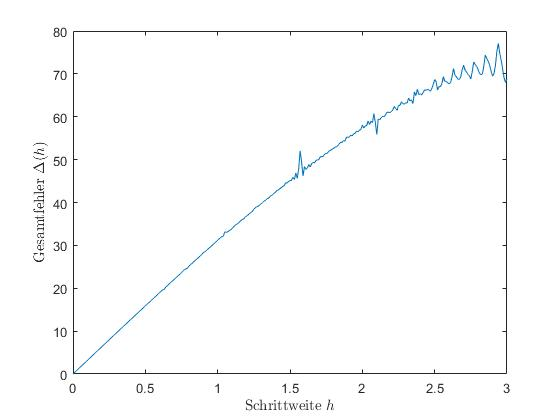
\includegraphics[scale=0.5]{frstplt_latex.jpg}
	\caption{Gesamtfehler $\varDelta(h)$ über Schrittweite $h$} 
\end{figure}


\newpage

\section{Lokaler Fehlerplot}

Es ist zu erkennen, dass der lokale Fehler $E_h$ mit steigender Schrittweite $h$ steigt. Jede der Kurven lässt eine Schwebung erkennen. Eine Betrachtung der abgebildeten Funktion liefert die Erklärung:
\[
f(x)\coloneqq \cos(x) - \frac{\sin(x+h)-sin(x)}{h}
\]
Der hintere Teil kann aufgefasst werden als Linearkombination der harmonischen Schwingungen $f_1(x)=\frac{1}{h} \sin(x+h)$ und $f_2(x)=\frac{1}{h}\sin(x)$. Additionstheoreme liefern: 
\[
f_1(x)-f_2(x)=2\cos\left(\frac{x+h}{2}\right)\sin\left(\frac{x-h}{2}\right)
\]  
Darüber hinaus lässt sich ablesen, dass mit steigendem $h$ der lokale Fehler $E_h$ steigt, was direkt eine Erhöhung der Amplitude der Einhüllenden zur Folge hat. Der $\cos(x)$-Term ist hierbei jeweils nur ein sich verändernder Offset.
\begin{figure}[ht!]
	\centering
	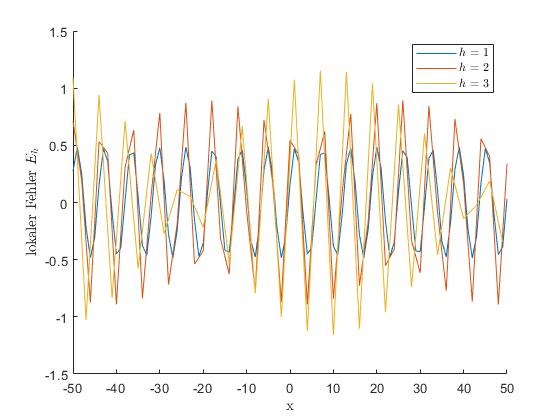
\includegraphics[scale=0.5]{scndplt_latex.jpg}
	\caption{Lokaler Fehler $E_h$ über $x$ für Schrittweiten für $h \in \{1,2,3\}$}
\end{figure}



\end{document}